\documentclass[12pt,a4paper]{extreport}
\usepackage{epsfig}
\usepackage{moreverb}
\usepackage{color}
\usepackage{fancyhdr,a4wide}
\usepackage{makeidx}
\usepackage{amssymb,amsmath}
\usepackage{multirow}
\usepackage{fancyvrb}
\usepackage{listings} 
\usepackage[ngerman,english]{babel}
\usepackage{graphicx}
\usepackage{url}
\usepackage[pdffitwindow=true,pdfstartview=Fit]{hyperref}
\usepackage{amssymb,amsmath}
\usepackage[nonumberlist,acronym,toc]{glossaries}
\usepackage[all]{hypcap}

\makeglossaries
\newacronym{IR}{IR}{Information Retrieval}
\newacronym{LSA}{LSA}{Latent Semantic Analysis}
\newacronym{CMS}{CMS}{Content Management Systems}
\newacronym{LSI}{LSI}{Latent Semantic Indexing}
\newacronym{SVD}{SVD}{Singular Value Decomposition}
\newacronym{VSM}{VSM}{Vector Space Model}


% don't indent new paragraphs
\parindent 0pt

\hoffset+0.3in
\textwidth13cm
\textheight22cm

\usepackage{graphicx}
\makeatletter
\def\ScaleIfNeeded{%
\ifdim\Gin@nat@width>\linewidth
\linewidth
\else
\Gin@nat@width
\fi
}
\makeatother

\pagestyle{headings}
\begin{document}
\clubpenalty = 10000
\widowpenalty = 10000 
\displaywidowpenalty = 10000

\newenvironment{summary}{\begin{quotation}\it\textbf{Summary.\space}}{\end{quotation}\vspace{0.3cm}}
\begin{titlepage}
\begin{minipage}{1\linewidth}
\begin{flushright}
\begin{minipage}[h]{0.4\linewidth}

\includegraphics[height=2cm]{img/STSlogo}
\end{minipage}
\hspace{0.5cm}
\begin{minipage}[h]{0.4\linewidth}

\includegraphics[height=2cm]{img/CoremediaLogo}
\end{minipage}\\
\bigskip
\Huge
\hrulefill\\
\bigskip
Tag Cloud Control \\by Latent Semantic Analysis\\
\hrulefill\\ \bigskip \bigskip
\normalsize submitted by\\
\large
Angelina Velinska\\
\vspace{0.5cm}
\end{flushright}
\end{minipage}

\vspace{5.5cm}

\begin{minipage}[b]{1\linewidth}
\begin{flushright}
\bigskip


\end{flushright}
\end{minipage}

\begin{minipage}[b]{1\linewidth}
\begin{flushright}
\bigskip 
%\bigskip
supervised by\\
\large
Prof. Dr. Ralf M\"oller\\
Dipl. Ing. Sylvia Melzer\\
\bigskip
Software Systems Institute (STS)\\
Technical University of Hamburg-Harburg\\
\bigskip
Dr. Michael Fritsch\\
%\bigskip
CoreMedia AG\\
Hamburg\\
\bigskip 
\bigskip
\end{flushright}
\end{minipage}

\end{titlepage}

% include after creating the abstract
%\begin{abstract}

A short description of my work. 

\end{abstract}


% don't put page numbers on declaration and acknowledgement pages:
%{\renewcommand{\thepage}{}
%\bigskip
\bigskip

\pagebreak\par
{\LARGE\noindent \textbf{Declaration}}\\

\bigskip
\bigskip

\noindent I declare that:\\

\medskip

This work has been prepared by myself, all literal or content based quotations are clearly pointed out, and no other sources or aids than the declared ones have been used.\\
\vspace{2cm}\\

\begin{flushright}
Angelina Velinska 
\end{flushright}

Hamburg \\
December, 2010 

\pagebreak 

%\pagebreak\\
\vspace{14cm}\\

Thank you...



\pagebreak

%}


% make figure names bold:
\makeatletter
\renewcommand{\fnum@figure}{\textbf{Figure~\thefigure}}
\makeatother

\tableofcontents
\listoffigures

\chapter{Introduction}
\label{sec:introduction}

Identifying the main concepts in texts is the subject of many research studies in the field of information retrieval and data mining. \\

This work investigates the implementation of Latent Semantic Analysis (LSA) for discovering the main concepts in texts, in order to present an overview of the text content in the form of a tag cloud.\\
\\
1. introductory words, why is this work being written \\
2. mention information retrieval, lsa, tag clouds - generally\\
3. mention cms ? document collections ? content ? \\
4. mention the work of david mugo \\
\\
During the last decade there have been constant optimizations in information retrieval effectiveness, making web search the preferred source of finding information. A substantial part of information retrieval deals with providing access to unstructured information in various domains. \gls{IR} refers to finding material (usually documents) of an unstructured nature (usually text) that satisfies an information need from within large collections (usually stored on computers) \cite{Mann08}. Many people today use methods from the field of IR when they use a search engine online, or search through their emails. In this context "unstructured data" refers to data which does not have a clear structure.\\

\gls{IR} technologies find wide application - in search engines, for browsing or filtering document collections, for further processing a set of retrieved documents. Before retrieval the documents are indexed, otherwise at each search, they would have to be scanned through for each query. The index maps the words or terms back to the documents where they occur. A method for document indexing, which is applied in this work, is called \gls{LSA}. It indexes the document collection by representing it as a reduced matrix of words and documents. \gls{LSA} representation improves \gls{IR} performance with respect to a basic problem of word-matching search - synonymy, or the case when more than one term describe the same concept. \\

While \gls{IR} deals with retrieval of documents, other systems manage content, such as documents. Content management includes a set of technologies and processes that support the creation, management and publication of content in any form or medium. Content may be documents, multi-media files, or any other file types that follow content lifecycle and require management. \gls{CMS} vary depending on their purpose and target environments - there are \gls{CMS} for the web, for enterprise, for mobile devices, as well as \gls{CMS} for managing collection of documents. \\

\section{Motivation and objective}
\label{sec:introduction:motandobj}  
A drawback of the classical \gls{LSA} implementation as an \gls{IR} method is the low precision of the returned results. A previous work by David Mugo \cite{mugo10} has investigated the improvement of \gls{LSA} precision performance by annotating the document collection and including the anotations used in \gls{LSA}. In his work, Mugo constructs a concept-document matrix from the annotations used, and concatenates it with the word-document matrix normally generated in \gls{LSA} process. The proposed solution, however, results in a slow speed of \gls{LSA}, and has left Mugo's hypothesis open. \\

Taking into consideration the results from Mugo's work, the current project has several objectives to reach. It will investigate the implementation of \gls{LSA} method for improving information retrieval in a domain-specific document management system with respect to context-based search. A further investigation will be made on improving the precision performance of \gls{LSA} method by using semantic annotations, and on finding an adequate way to present the results of \gls{LSA} as a tag cloud. And finally, it will be investigated how to use the tag cloud as a form of a relevance feedback to control \gls{LSA} method. \\

In the context of the stated objectives, semantic annotations are meta data annotations used to add information to unstructured data, or to the document collection. Semantic annotations are based on an ontology in our case, specifically developed for the domain of interest CoreMedia \gls{CMS}. Ontologies are used to capture some knowledge about a certain domain, by describing the concepts of the domain and the relationships between them. To further clarify the objectives, relevance feedback is an \gls{IR} technique, used to influence the retrieved results based on the user's preference. It allows the user to modify the initial tag cloud by selecting the most relevant words. The tag cloud is then re-generated from \gls{LSA} results with the relevance feedback posted as a query. \\

\section{Outline}
\label{sec:introduction:outline}
The reminder of this work is organized as follows. Chapter \ref{sec:docmanagsystem} describes in more detail what a document management system is, and provides an overview of the general structure of DocMachine 2.0, the \gls{CMS} deployed at CoreMedia AG. Chapter \ref{sec:semannot} presents the basic concepts of ontologies and document annotations based on ontologies. In Chapter \ref{sec:lsa} an overview of latent semantic analysis method is given, as well as an approach for improving \gls{LSA}'s precision by including semantic annotations in the method. Chapter \ref{sec:implementation} presents the prototype implementation and makes an evaluation of the results achieved in this work. And finally, conclusions are drawn in Chapter \ref{sec:conclusion}, along with some limitations of the current study and outlook for a future research.   \\ 

\chapter{Latent Semantic Analysis}
\label{sec:lsa}

%\begin{summary}
%The chapter gives a theoretical overview of \gls{LSA} in the context of its use in this work.
%\end{summary}
 
\section{Information Retrieval process}
\gls{IR} systems aim to satisfy user's information needs, by providing access to large collections of documents.  In a search application, the \gls{IR} process retrieves a set of documents which matches a given query. There are three basic processes which an \gls{IR} system has to support: to represent the content of the documents, to represent the user's information need, and to compare the two representations, based on a chosen similarity measure~(fig.~\ref{lsa:fig:ir_process}).
%
% IR process
%
\begin{figure}[htbp]
	\centering
	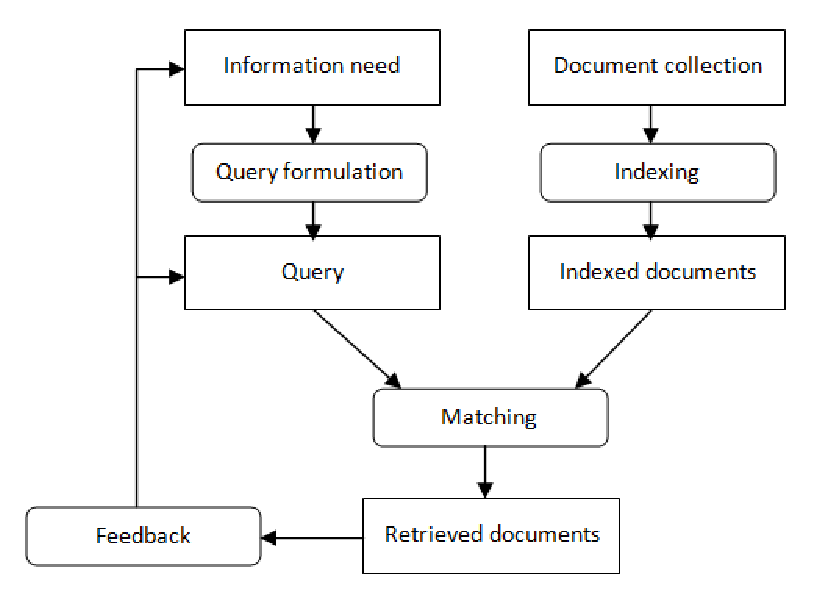
\includegraphics[scale=0.7]{img/IR} 
	\caption[Information Retrieval process]%
           {Information retrieval process, adapted from \cite{IRmodels09}. The information need of the user is formulated as a query, which is transformed in the chosen model of the \gls{IR} system. Documents from the collection are also represented according to the chosen model. Based on the implemented similarity measure, matching documents are identified. Finally, the retrieved results are presented to the user. If the user is not satisfied with the search results, the search query can be reformulated during feedback.}
\label{lsa:fig:ir_process}
\end{figure} 
Therefore, the first stage of constructing an \gls{IR} system is to extract information about the documents content, and implement a similarity measure, based on which documents and queries can be compared. Representing the documents is usually called the \textit{indexing process}. The comparison of the query against the document representations based on a chosen measure is called the \textit{matching process}.\\

\section{Document representation}
\label{sec:lsa:doc_repres}
In order to find documents which are similar to a given query, both documents and query have to be comparable, or have the same representation in the \gls{IR} system. Various models have been proposed for internal representation of documents and queries. The \textit{Boolean}, \textit{Vector space} and \textit{Probabilistic models} are popular \gls{IR} models that find wide implementation. The Boolean model represents both documents and queries as a set of terms, and compares them based on boolean functions ($AND$, $OR$, $NOT$, etc.). The probabilistic model uses probabilistic inference for document retrieval~\cite{probabilistic77}. Similarities are computed as probabilities that a document is relevant for a given query. And finally, the \gls{VSM}, introduced first by Salton~\cite{VSM_Salton89}, represents both documents and queries as vectors in a multidimensional space, whose dimensions are the terms used to build an index to represent the documents (section~\ref{section_vsm} provides more details on \gls{VSM}). Boolean model is easy to implement; however, when querying, users need to be familiar with boolean operators, which is a drawback of this model. Concerning the probabilistic model, prior knowledge is required for its implementation, as it usually includes tuning of independent probabilistic parameters. \gls{VSM} and the probabilistic model both have the advantage that they rank the relevant results according to a chosen weight function, but the former is easier to implement. \\

\subsection{Vector Space Model}
\label{section_vsm}
During indexing~(fig.~\ref{lsa:fig:ir_process}), documents are presented as data structures in memory. In \gls{VSM} a document is a vector, whose elements represent  properties like term frequencies, or frequency of word occurrence within the document. Before documents can be represented as vectors, they have to be tokenized, or converted from a stream of characters to a stream of words. Thus parsed, words will be used in building an index of the document collection. During tokenization one can apply filtering, i.e. removing HTML tags or other markup from text, as well as stop-words and punctuation marks removal. Stop words are such words that don't convey information specific to the text corpus, but occur frequently, such as: $ a, an, and, any, some, that, this, to $. \\
%
% vsm
%
\begin{figure}[H]
	\centering
	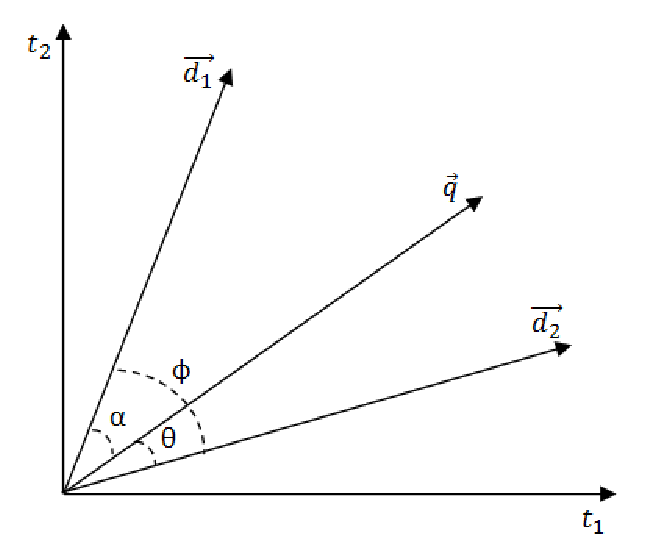
\includegraphics[scale=0.7]{img/vsm} 
	\caption[The Vector Space Model]%
           {The Vector Space Model. Documents $\vec{d_{1}}$ and $\vec{d_{2}}$, and a query vector $\vec{q}$ are represented in a two-dimensional vector space, formed by terms $t_{1}$ and $t_{2}$.}
\label{fig_vsm}
\end{figure}

A distinction has to be made between words or terms, and tokens. A term is the class which is used as a unit during parsing, and a token is each occurrence of this class. For example, in the sentence: 

\begin{quote}
\textit{CoreMedia CMS is shipped with an installation program for interactive graphical installation and configuration of the software.}
\end{quote}

the term $ installation $ is represented by two tokens. There is no universal way to parse a text, and the parsing decisions to address depend on the application in which the text collection will be used. \\

After tokenization, documents are represented as vectors, where each term is a vector in the vector space, and the documents are the sum of the terms, from which they consist. Thus, all document vectors and terms form a multi-dimensional vector space, where terms are the dimensions, and documents - the corresponding sum vectors. A diagram of the vector space is given in fig.~\ref{fig_vsm}, where two document vectors $\vec{d_{1}}$ and $\vec{d_{2}}$, and a query vector $\vec{q}$ are represented in a two-dimensional space. \\

\subsection{Weight functions}
\label{lsa:weight_functions}
Vectors in the \gls{VSM} have as elements the occurrence frequencies of words in documents. However, some documents are shorter than others, therefore one has to apply a normalization function in order to avoid representing words from longer documents as "more important" than words from shorter documents, as they would occur more often. Such normalization functions are called weight functions, and they are applied after the vector space has been constructed. \\

Weight functions are generally separated into two categories - local and global. They are often implemented as a pair together, because local functions measure the importance of a given word in a single document, while global functions give the importance of a word in the whole document collection. The most commonly used function pair is \textit{term frequency} and \textit{inverse document frequency}. \\

\subsubsection{Term frequency - inverse document frequency}
\label{lsa:tf-idf-section}
The simplest local weight is the term frequency $tf_{t,d}$. It assigns a weight to each term equal to the number of occurrences of the term $t$ in a given document $d$. However, not all words carry the same meaning in text (therefore, stop words are removed during preprocessing, as mentioned in~\ref{section_vsm}). Words that are common to all documents in the collection don't reveal much information, as compared to words which occur only in several documents. The latter are more likely to contain key information about the meaning of these documents.  This is reflected by the weight function \textit{inverse document frequency}~(eq.~\ref{lsa:idf})
\begin{equation}
\label{lsa:idf}
idf_{t}=1 + log\frac{N}{df_{t}}
\end{equation}

where $N$ is the total number of documents in the collection, $df_{t}$ is the frequency of occurrence of term $t$ in the whole collection, and $t$ is a specific term being weighted. Using $idf_{t}$ is a way to scale down the importance of commonly used words in text. When one combines both $tf$ and $idf$, a composite weight is produced for each term in each document. The \textit{tf-idf} weighting function assings to a term $t$ in a document $d$ a weight given by 
\begin{equation}
\label{lsa:tf_idf}
(tf-idf)_{t,d}=tf_{t,d} \times idf_{t}
\end{equation}. 

As defined by Manning et al.~\cite{IRbook2008}, the weight assigned to term $t$ in document $d$ by using a combination of local and global weight function is 
\begin{enumerate}
\item highest when $t$ occurs many times within a small number of documents;
\item lower when the term occurs fewer times in a document, or occurs in many documents;
\item lowest when the term occurs in virtually all documents.
\end{enumerate} 

\subsubsection{Log - entropy}
\label{lsa:log-entropy-section}
Another popular pair of weight functions, frequently used in text analysis, is the \textit{log-entropy} pair. The local function \textit{log} takes the logarithm of the raw term frequency, thus normalizing the effect when large differences in term frequencies occur. In eq.~\ref{lsa:log} $L(t,d)$ denotes the log of number of occurrence of a term $t$ in a document $d$. \\
% log
\begin{equation}
L(t,d)=\log(tf(t,d)+1)
\label{lsa:log}
\end{equation}

The global function \textit{entropy} $H(t)$ reflects the local relative importance of a term $t$ in the whole document collection~(eq.~\ref{lsa:entropy}) \\

% entropy
\begin{equation}
H(t) = 1+\frac{{\Sigma_{j}p(t,d)}}{\log n}
\label{lsa:entropy}
\end{equation}
where $n$ is the number of documents in the whole collection. In eq.~\ref{lsa:entropy}, $p(t,d)$ is defined by:
% entropy
\begin{equation}
p(t,d) = \frac{tf_{t,d}}{gf_{t}}
\end{equation}

where $gf_{t}$ is the total number of times that term $t$ occurred in all documents. The entropy measures the distribution of terms over all documents. \\

\subsection{Similarity measures}
\label{lsa:similarity_measures}
Once the vector space has been built, one can find the documents which are most similar to a given query. During \textit{query formulation}(fig.~\ref{lsa:fig:ir_process}), the queries are tokenized and represented as vectors, as already described in section~\ref{section_vsm}. Therefore, the similarities between documents and queries can be measured based on the angles between their respective vectors~(in fig.~\ref{section_vsm}, these are $ \alpha $ and $ \theta $). Using the angles between vector representations, one can define a similarity measure which is necessary for the matching process in \gls{IR} systems. The standard way to computing the similarity between two documents $d_{1}$ and $d_{2}$ is to compute the \textit{cosine similarity} of their vector representations $\overrightarrow{d_1}$ and $\overrightarrow{d_2}$ ~(eq.~\ref{lsa:cosine_measure}).

%
% cosine similarity
%
\begin{equation}
\label{lsa:cosine_measure}
sim(d1,d2)=\frac{\overrightarrow{V}(d_1).\overrightarrow{V}(d_2)}{\left\vert \overrightarrow{V}(d_1) \right\vert.\left\vert \overrightarrow{V}(d_2)\right\vert},
\end{equation}

where the numerator represents the \textit{dot product}\footnote{The dot product $\overrightarrow{x}.\overrightarrow{y}$ of two vectors is defined as $\displaystyle\sum\limits_{i=1}^{M} x_{i}y_{i} $.} of the vectors, while the denominator is the product of their \textit{Euclidean lengths}\footnote{Let $\overrightarrow{d}$ is the document vector for $d$, with $M$ components $\overrightarrow{d_{1}}...\overrightarrow{d_{M}}$. The Euclidean length of $d$ is defined to be $ \sqrt{\sum\limits_{i=1}^{M} \overrightarrow{d_{i}^2}} $}. The measure from eq.~\ref{lsa:cosine_measure} is the cosine of the angle $ \phi $ between the two vectors $\overrightarrow{d_1}$ and $\overrightarrow{d_2}$. \\

Once we represent a collection of $N$ documents as a collection of vectors, it is easy to obtain a natural view of the collection as a \textit{term-document matrix}: this is a $m \times n$ matrix whose rows represent the $m$ terms in the document collection, and each of whose $n$ columns corresponds to a document. And this specific matrix grouping all documents and terms from the collection is used in \textit{Latent Semantic Analysis}, a technique which is discussed next.\\

\section{Latent Semantic Analysis}
\gls{LSA} was first introduced by Dumais et al.~\cite{Dumais88usingLSA} and Deerwester et al.~\cite{Deerw90_LSA} as a technique for improving information retrieval. It is based on the Vector Space Model, where as already discussed, words from users' queries are matched with the words in documents. Such \gls{IR} models that depend on lexical matching have to deal with two problems: \textit{synonymy} and \textit{polysemy}. Due to the many meanings which the same word can have, also called polysemy, irrelevant information is retrieved when searching. And as there are different ways to describe the same concept, or synonymy, important information can be missed. \gls{LSA} has been proposed to address these fundamental retrieval problems, having as a key idea dimension reduction technique, which maps documents and terms into a lower dimensional semantic space. \gls{LSA} models the relationships among documents based on their constituent words, and the relationships between words based on their occurrence in documents. By using fewer dimensions than there are unique words, \gls{LSA} induces similarities among words including ones that have never occurred together~\cite{Dumais2006}. The basic steps in using \gls{LSA} are: document representation (the same as in \gls{VSM}), \gls{SVD} with dimensionality reduction, and querying. Next, the theoretical basis for \gls{LSA} is given, as it has been implemented as a part of this work. \\


As mentioned above, the first step of \gls{LSA} implementation is document representation. It is similar to the representation in \gls{VSM}, therefore refer to section~\ref{sec:lsa:doc_repres}. After tokenizing all documents in the collection, and computing the corresponding term weights, one has to construct a term-document matrix~(eq.~\ref{lsa:sparse_matrix_A}). Having as rows the terms, and as columns the documents, its elements are the occurrences of each term in a particular document, where $ a_{ij} $ denotes the frequency with which term $ i $ occurs in document $ j $. The size of the matrix is \text{\bf{m x n}}, where {\bf m} is the number of terms, and {\bf n} is the number of documents in the text collection. Since every term doesn't appear in each document, the matrix is usually sparse. \\

%
% initial sparse matrix A
%
\begin{equation}
A=
\begin{bmatrix}
\label{lsa:sparse_matrix_A}
 a_{11}& a_{12}& \cdots& a_{1n} \\
 \vdots& \vdots& \ddots& \vdots \\ 
 a_{m1}& a_{m2}& \cdots& a_{mn}
\end{bmatrix}
\end{equation}\\

Local and global weightings are applied to increase or decrease the importance of terms within documents. After presenting the most popular weight functions in sections~\ref{lsa:weight_functions}, we can write
%
% general weighting function
%
\begin{equation}
\label{lsa:global_local_weighting}
a_{ij}=L(i,j) \times G(i),
\end{equation}

where $L(i,j)$ is the local weighting of the term $i$ in document $j$, and $G(i)$ is the global weighting for term $i$. As examples of local functions, the term frequency $tf$ and $log$ were discussed, while $idf$ and entropy were the examples for global weightings. The choice of weight function impacts \gls{LSA} performance. In section~\ref{sec:lsa:factors_infl_lsa} reasons are given for the specific implementation decisions made in this work concerning \gls{LSA}. \\

\section{Singular Value Decomposition}
\label{sec:lsa:svd}

After its generation, the term-document matrix is decomposed into three matrices~(eq.~\ref{lsa:svd}) by applying \gls{SVD}. It is a unique decomposition of a matrix into the product of three matrices - $U$, $V$ and $\Sigma$, where $U$ and $V$ are orthonormal matrices\footnote{An orthonormal matrix is a matrix, whose columns, treated as 
 vectors, are also orthonormal. A matrix is orthonormal, if its transpose is equal to its inverse. For more information on matrices and matrix operations, refer to~\cite{MatrixCompGolub96}}, and $ \Sigma $ is a diagonal matrix\footnote{A diagonal matrix is a square matrix, in which the entries outside the main diagonal are all $0$.} having singular values\footnote{For a square matrix $A$, the square roots of the eigenvalues of $A^{T}A$, where $A^{T}$ is the conjugate transpose, are called \textit{singular values}. Given a matrix $A$, a non-zero vector $x$ is defined to be an \textit{eigenvector} of the matrix, if it satisfies the \textit{eigenvalue equation}: $Ax=\lambda x$ for some scalar $ \lambda $. The scalar $ \lambda $ is called an \textit{eigenvalue} of $A$ corresponding to the eigenvector $x$.\cite{MatrixCompGolub96}} on its diagonal.\\
%
% SVD decomposition in three matrices
%
\begin{equation}
\label{lsa:svd}
A=U \Sigma V^{T}
\end{equation}

After the initial matrix $A$ is decomposed, all but the highest $k$ values of its product diagonal matrix $\Sigma$ are set to $0$. When $A$ is recomputed again following eq.~\ref{lsa:svd}, the resulting  matrix $A_{k}$ represents the semantic space of the text collection. A classical visual example can be used to presenting \gls{SVD}~(as given in \cite{Dumais88usingLSA}) into three product matrices. It can be seen here how the dimensionality reduction of matrix $\Sigma$ affects all three product matrices.\\
%
% diagram of the truncated SVD
%
\begin{center}
\begin{figure}[htbp]
	\centering
	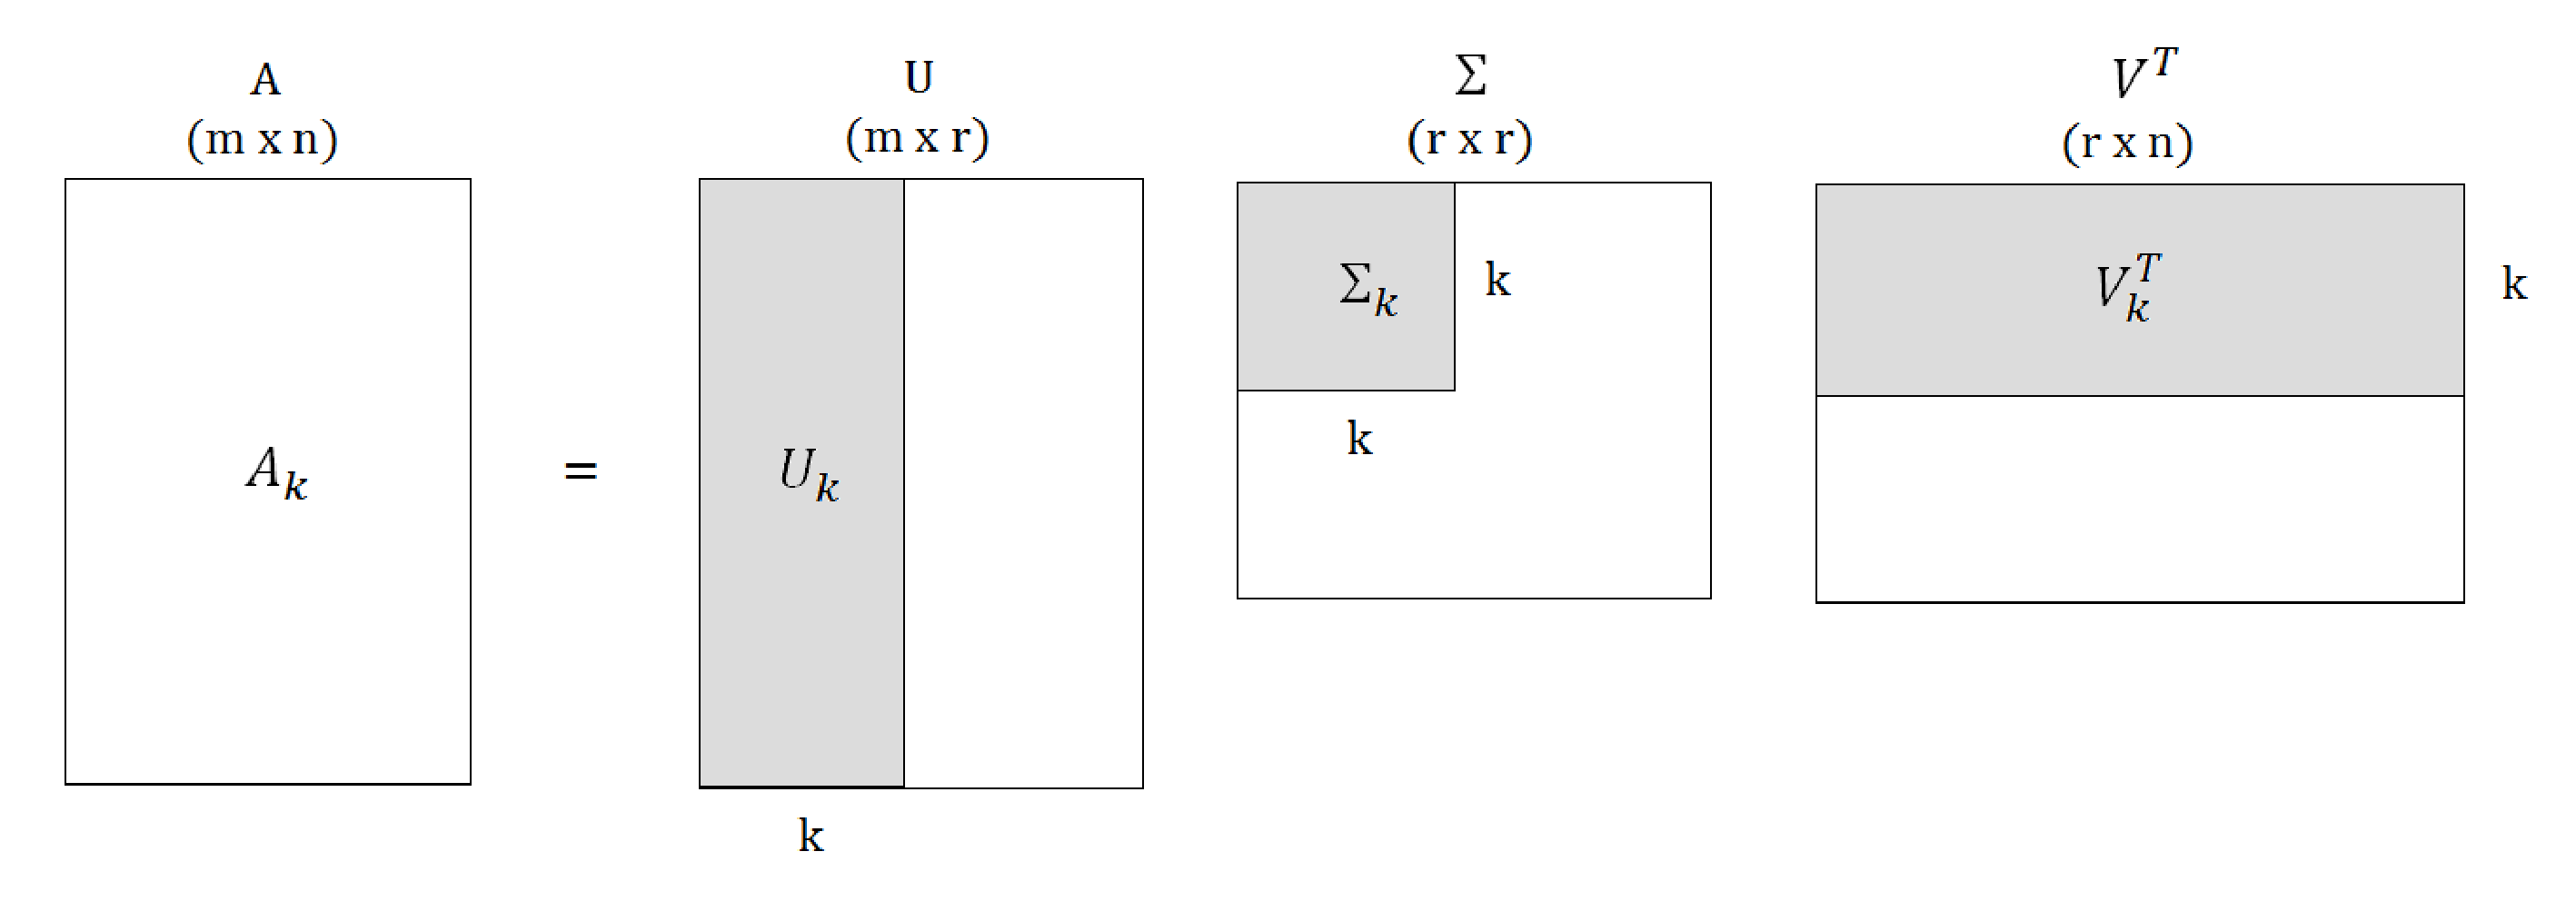
\includegraphics[width=\ScaleIfNeeded]{img/svd} 
 % or [scale=0.5]
	\caption[Diagram of truncated SVD]%
           {Diagram of truncated SVD}
\label{lsa:truncated_svd}
\end{figure}
%
% description of the parameters in SVD diagram
%
\begin{tabular}{l l}
$A_{k}$ - best rank-$k$ approximation of $A$ & $m$ - number of terms\\
$U$ - term vectors & $n$ - number of documents \\
$\Sigma$ - singular values & $k$ - number of factors \\
$V^{T}$ - document vectors & $r$ - rank of $A$ \\
\end{tabular}
\end{center} 

In fig.~\ref{lsa:truncated_svd}, $U$ and $V$ contain the term and document vectors respectively, and $\Sigma$ is constructed by the singular values of $A$. An important property of \gls{SVD} is that the singular values placed on the diagonal of $\Sigma$ are in decreasing order. Hence, if all but the first $k$ singular values are set to $0$, the semantic meaning in the resulting space is preserved to some approximation $k$, while noise or variability in word usage, is filtered out. Noise in this case are the terms with lowest weights which carry little meaning. By using fewer dimensions $k$, \gls{LSA} induces similarities among terms including ones that have never occurred together. Terms which occur in similar documents, for example, will be near each other in the k-dimensional vector space even if they never co-occur in the same document. This means that some documents that do not have any common words with a given query may be near it in resulting k-space.\\

A factor to be considered when computing \gls{SVD} is the run-time complexity of the algorithm. For decomposition of very large matrices, it is $O(n^2k^3)$, where $n$ is the number of terms in the text corpus, and $k$ is the number of dimensions in semantic space after dimensionality reduction. Note that  $k$ is typically a small number between 50 and 350.\\

A more detailed description of \gls{SVD} can be found in \cite{Berry95usinglinear} and \cite{MatrixCompGolub96}.\\

\section{Querying the semantic space}
\label{lsa:querying_sspace}

In this work \gls{LSA} is used for \gls{IR} purpose. Therefore, the final step of applying the technique is to pose queries on the constructed semantic space. A query $q$ is a set of words which must be represented as a document in the k-dimensional space, in order to be compared to other documents. The user's query can be represented by using eq.~\ref{lsa:query}:
%
% Query translation for LSA
%
\begin{equation}
\label{lsa:query}
q = q^{T}U_{k}\Sigma_{k}^{-1}
\end{equation}\\
where $q$ is the set of words in the query, multiplied by the reduced term and singular values matrices. Using the transformation in~eq.~(\ref{lsa:query}), the query is ''mapped'' onto the reduced k-space. After the mapping, the resulting query vector can be compared to the documents in the k-space, and the results ranked by their similarity or nearness to the query. A common similarity measure used to compute similarity between the query and the document vectors is the cosine~(eq.~\ref{lsa:cosine_measure}). From the resulting document set, the documents closest to the query above certain threshold are returned as search results. \\

\section{Factors which influence LSA performance}
\label{sec:lsa:factors_infl_lsa}
The effective usage of \gls{LSA} is a process of sophisticated tuning. Several factors can influence the performance of the technique. These factors are pre-processing of texts~(removal of stop-words, filtering, stemming), frequency matrix transformations, choice of dimensionality $k$, choice of similarity measure. Dumais et al.~\cite{dumais91improving} and Nakov et al.~\cite{Nakov_weightfunctions} have carried out research on \gls{LSA} performance depending on the choice of the above mentioned factors. They conclude that \gls{LSA} performance depends on the particular text corpus, as well as on the purpose of \gls{LSA} application. However, in the case of matrix transform, log-entropy~(section~\ref{lsa:log-entropy-section}) performs better as compared to other matrix transform function combinations, including the popular term frequency - inverse document frequency~($tf-idf$)~(section~\ref{lsa:tf-idf-section}). Therefore, the former is implemented in this work. It has been further stated~(\cite{dumais91improving},\cite{NakovBetterResultsLSI}) that with respect to similarity measures used, \gls{LSA} performs optimal when cosine similarity measure is implemented to calculate the distance between vectors in the semantic space~(eq.~\ref{lsa:cosine_measure}). It is therefore used in this work to measure the relevance between queries and documents. And finally, the dimensionality reduction parameter $k$ is defined empirically based on the experimentation results presented in Chapter~\ref{chapter:evaluation}.

\chapter{Tag Clouds}
\label{sec:semannot}

\begin{summary}
This chapter presents an overview of tagclouds used as a method for representing text content.
\end{summary}

Tag Clouds are popular applications used for vaious purposes: as a navigation mechanism, as indicators of activity within social media experiences, for visualization in texts and textual data, for annotation of documents~\ref{fig:tagcloud}. The importance or weight of words in the tag cloud are shown with size of font and/or color. The tag clouds are hyperlinks leading to a collection of items associated with the tag.\\
A version of tag cloud is called text cloud. It is used as a visual display that conveys the broad themes that emerge from textual analysis.  
There are three types of tag clouds depeding on their purpose and use. The first type contains a tag represeting the frequency of each term. The second type is a global tag cloud whose tags has frequencies aggreggated over all items and users. The third type of tag cloud contains categories, and its tags' size indicates the number of subcategories.\\
%TODO
%generate a tag cloud based on the contents in docmachine!!!!!!! replace the figure
%
% Opencloud
%
\begin{figure}[htbp]
	\centering
	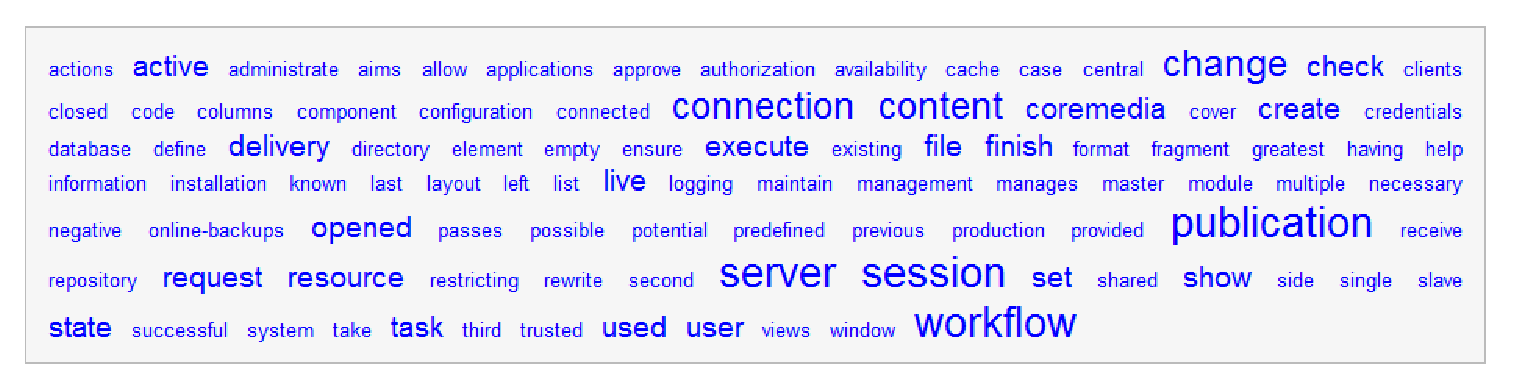
\includegraphics[width=\ScaleIfNeeded]{img/tagcloud} 
 % or [scale=0.5]
	\caption{Tag Cloud}
	\label{fig:tagcloud}
\end{figure}

\section{1}
\label{sec:semannot:1}
Related work 
SenseBot Search Results Summarizer is a plugin for Mozilla Firefox browser that generates a tag cloud of the main concepts returned as search results from Google.

LinkSensor
SenseBotSummarizer
All three are based on SenseBot - a semantic search engine.
Made available from Semantic Firefox Extensions \footnote{\url{http://www.semanticengines.com/plugins.htm}}


\chapter{Implementation}
\label{sec:implementation}

This chapter describes the implementation part of the thesis work. After presenting in Chapter~\ref{sec:lsa} the theoretical basis behind \gls{LSA}, and in Chapter~\ref{chapter:cluster_labeling} cluster labeling, theoretical application and specific implementation decisions are discussed here. All software tools and libraries which were used are pointed out, and code snipplets are given. Then in Chapter~\ref{chapter:evaluation}, test results are shown, and evaluation of the implementation is made. \\

\section{Clustering, labeling}
For the ontology development, we used Protege Ontology Editor 4.1~\footnote{\url{http://protege.stanford.edu/}, accessed December, 2010} from Stanfornd University. The ontology is a light-weight domain-specific ontology developed in OWL for CoreMedia \gls{CMS} domain. \\

\section{Tag Cloud implementation}
\label{sec:implementation:tag_cloud}
The implemented open source library used for tag cloud generation is called Opencloud\footnote{\url{http://opencloud.mcavallo.org/}, accessed December, 2010}, and is provided by Marco Cavallo.\\

Tag clouds can be generated automatically by using the most frequent words, by removing stop words, etc. preprosessing. They can also be custom made, by using important concepts retrieved after \gls{IR} task has been performed - e.g. on search results, on main concepts as in our case, based on concepts retrieved using \gls{LSA}. \\

\section{Tools used}
\label{sec:implementation:tools_used}
Airhead Research\footnote{\url{http://code.google.com/p/airhead-research/}} project was used as a semantic spaces Package which provides a java-based implementation of \gls{LSA}.\\

Apache Lucene\footnote{\url{http://lucene.apache.org/java/3_0_2/}, accessed December, 2010} was used as an indexing and search library.

\section{Advantages and drawbacks}
\label{sec:lsa:adv_disadv}

why am i using lsa instead of lda for example?\\

\begin{enumerate}
\item PLSA - characteristics, advantages, disadvantages
\item LDA - characteristics, advantages, disadvantages
\end{enumerate}


\chapter{Conclusion and outlook}
\label{sec:conclusion}

Search applications process huge amounts of information. Presenting this information to the users is an important part of these applications, and can improve their usability. We applied clustering as a method to organize search results into browsable groups of documents. In order to present these prepared groups of documents to the end users, informative and summarizing cluster labels are needed. Therefore, we evaluated the implementation of \gls{WCC} cluster labeling method, and outlined a proposal for its improvement. \\

With respect to the problem of how to present many search results to users, we implemented a tag cloud, which summarizes the main concepts in search results, thus acting as a visualization mean. 


\section{Future Work}
The goals set for this project and given in section~\ref{sec:goal_scope} were reached. The project can still be developed further. Below, we outline our proposals for future work. \\

\subsection{Implementation}

! Implement the prototype as a part of DocMachine\footnote{\url{https://documentation.coremedia.com/}} - the online documentation system at CoreMedia AG, Hamburg.

\subsubsection{LSA}
One of the major drawbacks in implementing \gls{LSA} is that computing \gls{SVD} for large matrices when applied to large document sets is computationally expensive. It has been stated that it is possible to compute \gls{SVD} in an incremental manner, and with reduced resources via neural-network like approach~\cite{brand06}. However, currently there is no Java-based implementation of this algorithm. As this project is developed using Java, it remains as future work to implement the fast incremental \gls{SVD} computation, proposed by Brand~\cite{brand06} in Java, in order to use it in this work. \\

\subsubsection{Cluster labeling}
Other clustering methods can be investigated, such as \gls{STC}, which preserves the word order in documents, by presenting them in the form of a tree. Cluster labeling using \gls{STC} involves also using phrases as candidate labels, instead of separate terms, which improves usability, as compared 
to the investigates \gls{WCC} algorithm. \\

\subsubsection{Cluster labeling using external knowledge}
Due to time constraints, it remains for future work to evaluate and present experimental results on running \gls{WCC} algorithm for cluster labeling with external knowledge from an ontology. \\

\subsection{Testing}
A larger set of document can be used for evaluation and testing of our implementation. In this work we carried out tests on a document set consisting only of 15 documents in 3 categories. Research has shown, however, that \gls{LSA} perform better when applied to document collections above 3000 documents, each of which larger than $\approx 60$ words, testing our implementation on a larger document collection remains as future work. \\



% prints the list of acronyms
% call: latex thesis, makeglossaries thesis, latex thesis
%
\printglossaries


\begin{appendix}
\chapter{Appendix}

You should not print the full source code :-). But note that the chapters are now called ``appendix'' and numbered with letters.

\end{appendix}

% After adding new references to the "references.bib" file, first invoke latex, then
% bibtex on the references file, then latex again:
% latex thesis
% bibtex thesis
% latex thesis

% number the bibliography instead of alpha-numerial abbrev.
%\bibliographystyle{alpha} 
\bibliographystyle{ieeetr}
\bibliography{references}
\end{document}
